\newpage
\section{Agenti basati su conoscenza}
C'è bisogno di rappresentare la conoscenza in maniera parziale e incompleta (gli ambienti sono parzialmente osservabili). Ci servono quindi dei linguaggi più espressivi e con \textbf{capacità inferenziali}.\\
\subsection{Knowledge Base}
L'insieme di tutta la conoscenza necessaria a decidere un'azione da compiore è la \textbf{knowledge base} e può essere definita in due modi:
\begin{itemize}
	\item \textit{Dichiarativo}: all'agente viene detto cosa deve sapere, partendo da una conoscenza di base vuota e aggiungendo progressivamente formule (TELL)
	\item \textit{Procedurale}: si scrive un programma che definisca il processo decisionale una volta per tutte
\end{itemize}

\begin{definition}[Knowledge Base]
	Un insieme di \emph{enunciati} (formule) espressi in un linguaggio di rappresentazione.
\end{definition}

\begin{example}[Wumpus World]
	\label{example:wumpus_world}
	Il mondo del Wumpus è una caverna fatta di stanze connesse tra loro. All'interno c'è questa bestia puzzolente che mangia chiunque entri nella stanza in cui si trova. Questo può essere ucciso dall'agente che ha una freccia a disposizione.\\
	Ci sono delle stanze con degli \textit{ostacoli}: pozzi, in cui se l'agente entra, muore. In una delle stanze si trova l'\textit{obiettivo}, ovvero un lingotto d'oro.\\
	L'agente non conosce l'ambiente e la sua posizione, se non all'inizio.
	\begin{center}
		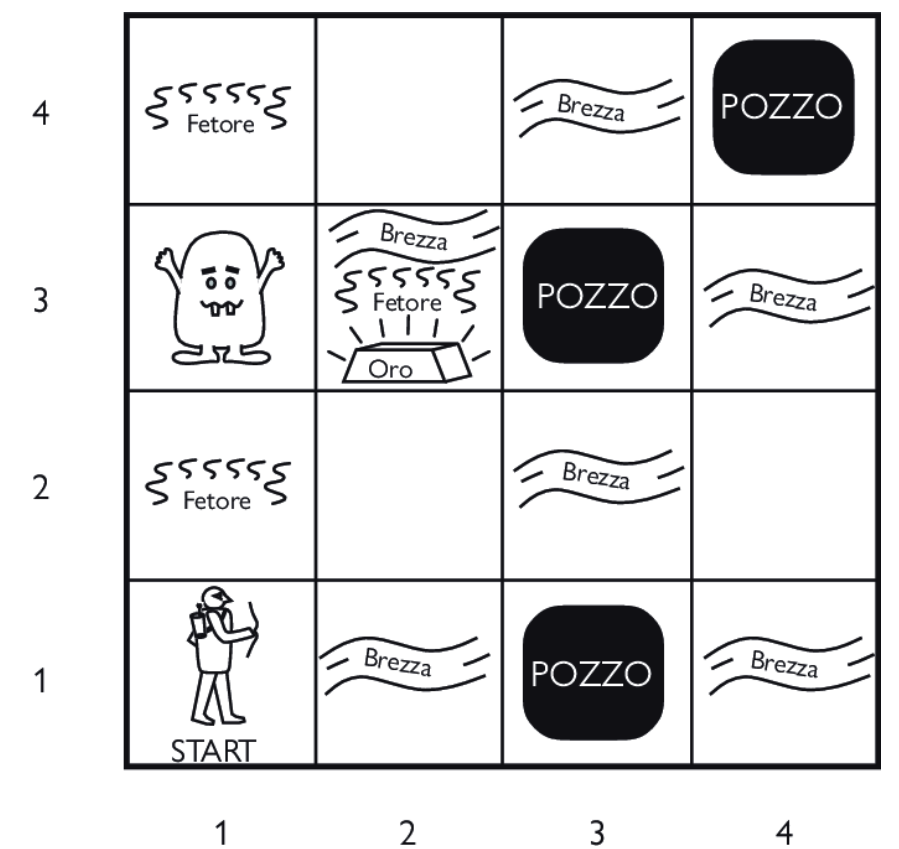
\includegraphics[scale=0.21]{wumpus_world.png}
	\end{center}
	Definiamo le \textbf{misure di prestazione}:
	\begin{itemize}
		\item +1000 se trova l'oro, torna in [1,1] ed esce
		\item -1000 se muore
		\item -1 per ogni azione
		\item -10 se usa la freccia
	\end{itemize}
	Invece l'\textbf{ambiente} è una griglia 4x4 circondata da pareti di delimitazione. L'agente inizia sempre nella posizione [1,1] rivolto verso destra (la prima casella è sempre safe). Le posizioni dell'oro e della bestia sono casuali e tutti i riquadri hanno una probabilità di $0.2$ di contenere un pozzo.\\
	L'agente può fare le seguenti \textbf{azioni}:
	\begin{itemize}
		\item Andare avanti
		\item Ruotare a destra o a sinistra di $90°$
		\item Afferrare un oggetto
		\item Scagliare la freccia
		\item Uscire
	\end{itemize}
	Il nostro agente puo \textbf{percepire} le seguenti cose:
	\begin{itemize}
		\item \textit{Fetore} nelle caselle adiacenti alla bestia
		\item \textit{Brezza} nelle caselle adiacenti ai pozzi
		\item \textit{Luccichio} nella casella con l'oro
		\item \textit{Urlo} se la bestia viene uccisa
	\end{itemize}
	e vengono rappresentati come una quintupla, che ad  esempio nella prima casella vale:
	\begin{equation*}
		[none,none,none,none,none]
	\end{equation*}
	Di conseguenza sappiamo che nelle caselle adiacenti non ci sono né pozzi né la bestia.
\end{example}

\subsubsection{Tell-Ask}
L'agente interagisce con la knowledge base tramite un'interfaccia funzionale di tipo Tell-Ask:
\begin{itemize}
	\item \textit{Tell}: aggiungere nuovi enunciati
	\item \textit{Ask}: interagire con la knowledge base
	\item \textit{Retract}: eliminirare enunciati
\end{itemize}
Gli enunciati nella KB rappresentano le credenze dell'agente e le risposte $\alpha$ devpomp essere tali per cui queste discendano necessariamente dalla KB.\\
Il problema fondamentale è quindi capire, data una base di conoscenza KB, come dedurre che un certo fatto $\alpha$ è vero di conseguenza.
\begin{equation}
	KB \models \alpha
\end{equation}
Un programma basilare è il seguente:
\begin{lstlisting}
	function Agente-KB (percezione) returns azione
		persistent: KB, una base di conoscenza
			t, un contatore, inizialmente a 0, che indica il tempo
		TELL(KB, Costruisci-Formula-Percezione(percezione, t ))
		azione = ASK(KB, Costruisci-Query-Azione( t ))
		TELL(KB, Costruisci-Formula-Azione(azione, t ))
		t = t + 1
		return azione
\end{lstlisting}
\subsubsection{Analisi}
A differenza di una \textit{base di dati}, la base di conoscenza non contiene solo fatti specifici da recuperare ma anche fatti generali, oregole, espressi in maniera esplicita in un linguaggio compatto. Questo le conferisce la \textbf{capacità inferenziale}, ovvero derivare nuovi fatti da quelli memorizzati.\\
Il lato negativo è che, avendo un linguaggi  più espressivo, è \textbf{meno efficiente} il meccanismo inferenziale. Serve quindi trovare il giusto bilanciamento da \textit{espressività} del linguaggio e \textit{complessità} del meccanismo inferenziale.

\subsection{Logica}
Le KB sono costituite da enunciati espresse secondo le regole della \textbf{sintassi}. La \textbf{semantica} invece ne esprime il significato. Un \textbf{modello} è una configurazione dei valori di verità che si possono assegnare alle variabili di una formula.
\subsubsection{Formalismo}
Un formalismo per la rappresentazione della conoscenza si compone di:
\begin{itemize}
	\item Una \textbf{sintassi}: un linguaggio composto da un vocabolario e da regole per la formulazione degli enunciati
	\item Una \textbf{semantica}: stabilisce una corrispondenza tra gli enunciati e ifatti del mondo
	\item Un \textbf{meccanismo inferenziale} che ci consente di inferire nuovi fatti
\end{itemize}
\begin{center}
	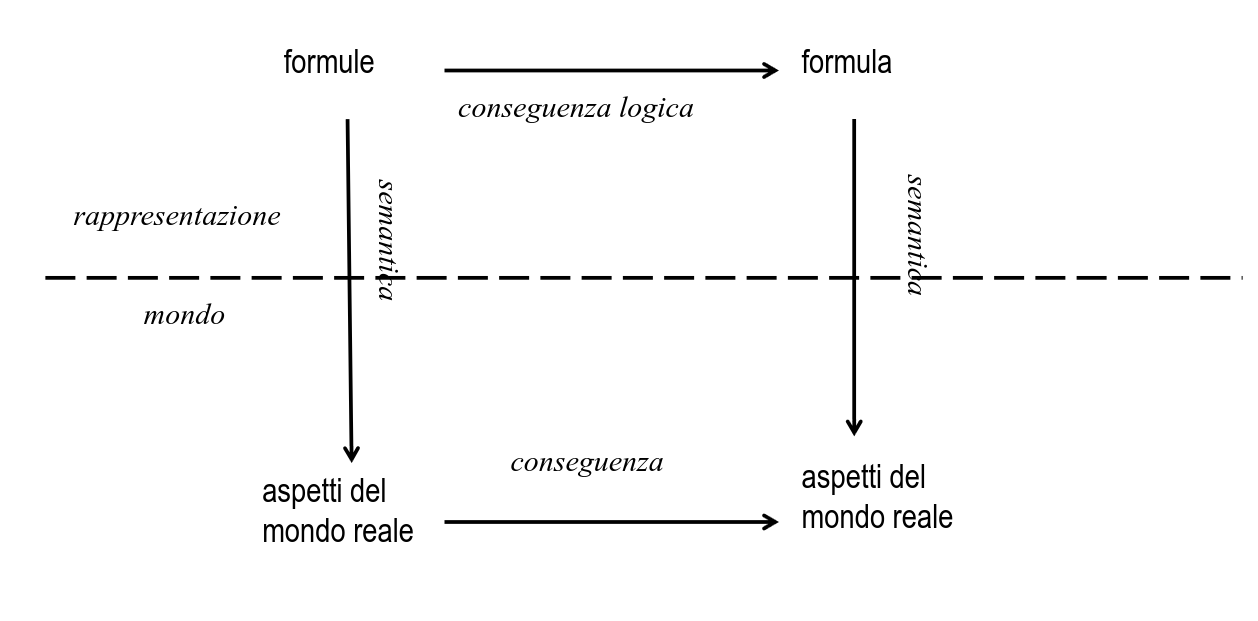
\includegraphics[scale=0.25]{formalismo.png}
\end{center}
Facendo il paragone con l'agente, le formule sono le sue configuraziini fisiche e il ragionamento è il processo di costruzione di nuove configurazioni a partire dalle vecchie. Il ragionamento logico deve assicurare che le nuove configurazioni siano effettive conseguenze sul mondo causate dalle vecchie configurazioni.

\subsection{Logica proposizionale}
\subsubsection{Sintassi}
La sintassi è la seguente, rappresentata in BNF:
\begin{equation}
	\begin{split}
		formula & \to formulaAtomica \vert formulaComplessa \\
		formulaAtomica & \to True \vert False \vert simbolo \\
		simbolo & \to P \vert Q \vert R \vert \ldots \\
		formulaComplessa & \to \neg formula \\
		&\vert (formula \land formula) \\
		& \vert (formula \lor formula)\\
		& \vert (formula \Rightarrow formula)\\
		& \vert (formula \Leftrightarrow formula)
	\end{split}
\end{equation}

\subsubsection{Semantica}
La logica proposizionale segue una semantica \textbf{composizionale}, dove il significato di una frase è determinato dal significato dei suoi componenti a partire dai \textit{simboli proposizionali}. Di seguito la ravola di verità:
\begin{table}[h!]
	\centering
	\begin{tabular}{|cc|ccccc|}
		\hline
		$P$ & $Q$ & $\neg P$ & $P \land Q$ & $P \lor Q$ & $ P \Rightarrow Q$ & $P \Leftrightarrow Q$\\
		\hline
		false & false & true & false & false & true & true \\
		false & true & true & false & true & true & false \\
		true & false & false & false & true & false & false \\
		true & true & false & true & true & true & true\\
		\hline
	\end{tabular}
\end{table}

\subsubsection{Conseguenza logica}
\begin{definition}[Conseguenza logica]
	Una formula $\alpha$ è una conseguenza logica di un insieme di formule KB se e solo se in ogni modello di KB, anche $\alpha$ è vera ($KB \models \alpha$).
\end{definition}
Indichiamo con $M(KB)$ i modelli dell'insieme di formule in KB e con $M(\alpha)$ l'insieme delle interpretazioni che rendono $\alpha$ vera, ovvero i suoi \textbf{modelli}.
\begin{equation}
	KB \models \alpha \Leftrightarrow M(KB) \subseteq M(\alpha)
\end{equation}

\subsubsection{Model checking}
Un modo per determinare la conseguenza logica è quello di enumere i \textit{modelli} e mostrare che la formula $\alpha$ vale in tutti quelli in cui è vera la KB.

\begin{example}[Wumpus World]
	Partendo dall'esempio \ref{example:wumpus_world} abbiamo che la KB iniziale, $KB_0$, è costituita dalle regole descritte nella definizione dell'esercizio:
		\begin{gather*}
			\neg W_{1,1} \quad \neg P_{1,1} \\
			B_{2,1} \Leftrightarrow (P_{1,1} \lor P_{2,2,} \lor P_{3,1})\\
			B_{1,1} \Leftrightarrow (P_{1,2} \lor P_{2,1})\\
			\vdots
		\end{gather*}
		Il primo passo dell'agente è spostarsi in $[2,1]$ dato che in $[1,1]$ non ha percepito niente. Abbiamno quindi:
		\begin{equation*}
			KB_1 = KB_0 \cup \{\neg B_{1,1}, B_{2,1}, \neg F_{1,1}, \neg F_{2,1}, \ldots\}
		\end{equation*}
		e rappresentiamo le domande sulla presenza o meno di pozzi come:
		\begin{equation*}
			\begin{split}
				KB_1 \models \neg P_{1,2} \\
				KB_1 \models \neg P_{2,2} \\
				KB_1 \models \neg P_{3,1} \\
			\end{split}
		\end{equation*}
		Sapendo da $KB_0$ che non ci sono pozzi nella casella $[1,1]$ e che c'è un pozzo nella stanza adiacente solo se ci percepisce la brezza, formuliamo le seguenti proposizioni:
		\begin{equation*}
			\begin{split}
				& B_{1,1} \Leftrightarrow (P_{1,2} \lor P_{2,1}) \\
				& B_{2,1} \Leftrightarrow (P_{1,1} \lor P_{2,2} \lor P_{3,1})
			\end{split}
		\end{equation*}
		e concludiamo che non c'è brezza in $[1,1]$ e c'è in $[2,1]$, ovvero $\neg B_{1,1}$ e $B_{2,1}$.\\
		Ci rimangono quindi tre configurazioni possibili dato che abbiamo:
		\begin{gather*}
			KB_1 \models \neg P_{1,2}\\
			KB_1 \models P_{2,2}\lor P_{3,1}
		\end{gather*}
		e sono quelle in cui i pozzi sono in $[3,1]$ oppure in $[2,2]$ oppure in entrambi.
\end{example}